\chapter{Experimental setup}\label{chapter:ExpSetup}
%TODO: move all information from Pros/cons in text and remove column from table!

In this chapter, details on the experimental setup for the upcoming analysis in \autoref{chapter:Results} 
% \comWB{chapterref; do a ctrl+r and search for all "backslash ref"} 
are presented. First, the training dataset and the main training setup for all model variants proposed in this work are discussed.  
Then, the evaluation datasets and metrics involved in the method comparisons are described in short. Finally, the semi-supervised tracker HODOR \parencite{athar2022hodor} and the unknown object segmentation algorithm INSTR \parencite{durner2021unknown} are shortly presented to help the reader understand the details behind experiments in \autoref{chapter:Results}.

\section{Training dataset}\label{chapter:Dataset}
The dataset used for training is a synthetic dataset created with BlenderProc \parencite{denninger2019blenderproc}. It consists of scenes of 10 subsequent frames from different vantage points resulting from a simulated camera movement. During dataset generation, the initial and final camera coordinates are sampled randomly from a range of possible values.
% , all belonging to a sphere over the pile of objects \comWB{not clear what "the pile of objects" is at this point}. 
Once the initial and final camera position are defined, a trajectory is formed and the 10 subsequent frames are sampled linearly along the path formed by the camera trajectory. Depending on the camera motion, objects may be partially occluded by other neighboring objects or may completely disappear between frames. \par

The dataset includes 989 sequences. In total, a number of 5 to 12 objects are present in each scene, similar to the dataset used to train INSTR \parencite{durner2021unknown}, the method serving as our single shot unknown object segmentation baseline. In practice, \gls{BlenderProc} scenes are generated by simulating a free fall of a number of objects sampled from the database on a table. As a result of the object free fall, some small objects may be completely hidden for the whole sequence if the objects end up in a pile. Therefore, in practice, there are cases where the model is trained in scenes with less than 5 objects visible. \par 


Most similar semi-supervised learning methods in the literature perform training on shorter sequences than the ones available in the training dataset. More specifically, it has been demonstrated that only a pair of neighboring frames and their annotations suffices for the model to learn temporal consistency.
% \comWB{not even that, you can also take static frames and augment, like hodor pre-training on coco edit: just saw that you mention this later, would rephrase the sentence here}. 
For example \parencite{meinhardt2021trackformer} have shown that during pretraining, not even a tracking dataset is necessary, as neighboring frames can be obtained just by applying augmentations to an input frame. However, during finetuning neighboring frames are sampled from the tracking data sequences in MOT17 \parencite{mot17} and MOT20 \parencite{mot20}.
%\comWB{ref, think its also possible with just static frame augs?}. 
We follow the last strategy and sample pairs of images instead of longer sequences from the original 10-frame sequences, since this choice results in more data sequences to use as data samples during training and is sufficient for our model to learn temporal consistency. \par 

The input images are not augmented with any standard image augmentation technique, since adding random noise or flipping increases the differences between neighboring frames to a level that hinders the model from recognising the same object in different sequences. However, scaling, rotations and occlusions are already naturally introduced in scenes during dataset generation from the simulated camera movement. Therefore, the only processing taking place with regard to the input images is a standard ImageNet-based normalisation. Though the images are not augmented, augmentation on a track level is performed during training by randomly sampling neighboring frames within the whole sequence length of the 10-frame sequences. \par

\vspace{12mm}

\begin{figure}[h!]
  \centering
  \begin{tabular}{@{}c@{}}
     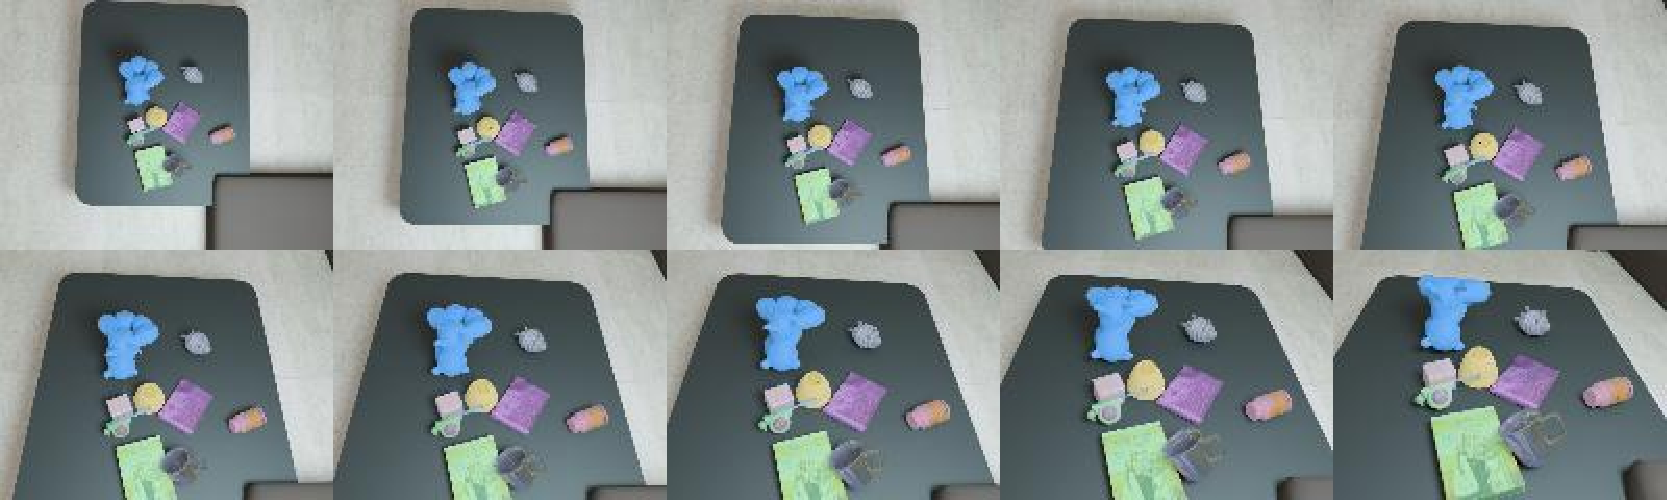
\includegraphics[width=1.\linewidth]{figures/03_method/easy_sequence.pdf}\\[\abovecaptionskip]
    \small (a) Sequence with slow camera movement, all samples remain visible in every scene
  \end{tabular}

  \vspace{0.5cm}

  \begin{tabular}{@{}c@{}}
    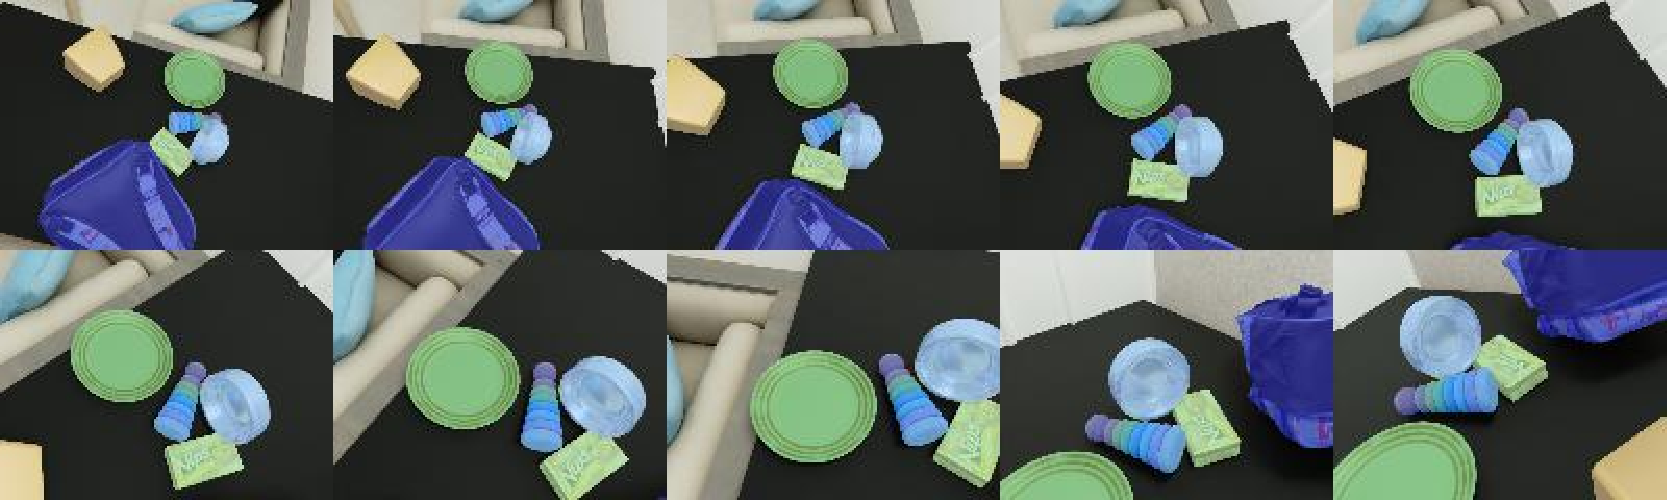
\includegraphics[width=1.\linewidth]{figures/03_method/hard_sequence.pdf}\\[\abovecaptionskip]
    \small (b) Sequence with faster camera movement that leads to occlusions
  \end{tabular}
    
  \caption{Training dataset overview 
  }\label{fig:dataset_overview}
\end{figure}


\section{Training setup}
For the training of the proposed model the setup described in \tabref\ref{Tab:training_setup} is followed.
%\comWB{don't quite get this}. 
Specifically, the dataset is loaded with a batch size of 2 and learning takes place with an AdamW optimizer. The learning rate is constant throughout the training and regularisation is ensured with a weight decay coefficient of $10^{-2}$. The number of images the loss is computed on (forward images) is 1 and the horizon is also set to 1, meaning that for each forward image also 1 neighboring frame is loaded during dataloading to learn temporal consistency. This short sequence length during training (total sequence length = 2 frames) has been proven to be effective in training trackers in numerous works like \parencite{meinhardt2021trackformer} and \parencite{savi}. Finally, the maximum number of tracked objects is restricted to 5, which means that in scenes with more object annotations, some objects are treated as part of the background. This setup choice helps ensure that the network learns to track only designated objects and not every object present in the scene, potentially preventing overfitting. \par

% \comWB{to strengthen your claim you could mention instr here, we claimed that the table presents a great cue to identify objects}\par



\begin{table} [h!]
\caption{Training setup}
\centering

\begin{tabular}{|c|c|} 
\hline
\textbf{Parameter}    & \textbf{Configuration} \\ 
\hline
batch size & 2   \\
optimizer  & AdamW \\
lr         & $10^{-5}$ \\
weight decay & $10^{-2}$ \\
num of fwd ims & 1 \\
min/max horizon & 1 \\
%max tracklet length & 1 \\
max classes & 5 \\
\hline
\end{tabular}
 \label{Tab:training_setup}
\end{table}

% All model variants compared in \autoref{seq:preliminary_exps} are trained with the aforementioned parameter choice. This ensures a more fair comparison between the available options to specify the best performing one to adopt as our final proposed method. 


\section{Evaluation datasets}
\subsection{Evaluation Test set}
For the method evaluation, a test set with longer sequences (minimum 50 frames) was generated with BlenderProc \parencite{denninger2019blenderproc}. The test set generation process resembles the training set generation with regard to the scene characteristics. More specifically, a random number of objects (5-12) and a random table were sampled from the database to form the scene. However, as already explained in section 4.1, from the nature of scene generation with BlenderProc that involves simulating objects falling on a table and forming a pile, some objects may end up completely invisible for the whole scene. Hence, scenes with less that 5 visible objects are also part of the test set. In the end, an equal number of crowded ($num\_of\_objs <6$) and not crowded ($num\_of\_objs >=6$) scenes were sampled to include in the test set. \par

\begin{table}
\centering
\small
\caption{Test set sequences overview}
\label{tabl:testset_overview}
\begin{tabular}{|c|c|c|c|c|c|c|}
\hline

   & Sequence names            & \begin{tabular}[c]{@{}l@{}}Num of \\ frames\end{tabular} & \begin{tabular}[c]{@{}l@{}}Num of \\ objects\end{tabular} & \begin{tabular}[c]{@{}l@{}}Visibility \\ score\end{tabular} & \begin{tabular}[c]{@{}l@{}}Type of \\ Movement\end{tabular} & Velocity \\
   \hline

0  & scene\_0\_zoom\_in\_slow & 100                                                      & 5                                                         & 0.99                                                         & zoom\_in                                                    & slow     \\
1  & scene\_0\_rotation\_slow & 100                                                      & 5                                                         & 0.97                                                         & rotation                                                    & slow     \\
2  & scene\_1\_zoom\_in\_slow & 100                                                      & 6                                                         & 0.99                                                         & zoom\_in                                                    & slow     \\
3  & scene\_1\_rotation\_slow & 100                                                      & 6                                                         & 1.00                                                         & rotation                                                    & slow     \\
4  & scene\_2\_zoom\_in\_slow & 100                                                      & 7                                                         & 0.76                                                         & zoom\_in                                                    & slow     \\
5  & scene\_2\_rotation\_slow & 100                                                      & 6                                                         & 0.70                                                         & rotation                                                    & slow     \\
6  & scene\_3\_zoom\_in\_slow & 100                                                      & 5                                                         & 0.57                                                         & zoom\_in                                                    & slow     \\
7  & scene\_3\_rotation\_slow & 100                                                      & 5                                                         & 0.70                                                         & rotation                                                    & slow     \\
8  & scene\_4\_zoom\_in\_slow & 100                                                      & 10                                                        & 0.77                                                         & zoom\_in                                                    & slow     \\
9  & scene\_4\_rotation\_slow & 100                                                      & 10                                                        & 0.78                                                         & rotation                                                    & slow     \\
10 & scene\_5\_zoom\_in\_slow & 100                                                      & 3                                                         & 1.00                                                         & zoom\_in                                                    & slow     \\
11 & scene\_5\_rotation\_slow & 100                                                      & 3                                                         & 1.00                                                         & rotation                                                    & slow     \\
12 & scene\_6\_zoom\_in\_slow & 100                                                      & 2                                                         & 0.87                                                         & zoom\_in                                                    & slow     \\
13 & scene\_6\_rotation\_slow & 100                                                      & 2                                                         & 0.94                                                         & rotation                                                    & slow     \\
14 & scene\_7\_zoom\_in\_slow & 100                                                      & 8                                                         & 1.00                                                         & zoom\_in                                                    & slow     \\
15 & scene\_7\_rotation\_slow & 100                                                      & 8                                                         & 1.00                                                         & rotation                                                    & slow     \\
16 & scene\_8\_zoom\_in\_slow & 100                                                      & 9                                                         & 0.95                                                         & zoom\_in                                                    & slow     \\
17 & scene\_8\_rotation\_slow & 100                                                      & 9                                                         & 0.95                                                         & rotation                                                    & slow     \\
18 & scene\_9\_zoom\_in\_slow & 100                                                      & 8                                                         & 0.67                                                         & zoom\_in                                                    & slow     \\
19 & scene\_9\_rotation\_slow & 100                                                      & 8                                                         & 0.84                                                         & rotation                                                    & slow     \\
20 & scene\_0\_zoom\_in\_fast & 50                                                       & 5                                                         & 0.98                                                         & zoom\_in                                                    & fast     \\
21 & scene\_0\_rotation\_fast & 50                                                       & 5                                                         & 0.97                                                         & rotation                                                    & fast     \\
22 & scene\_1\_zoom\_in\_fast & 50                                                       & 6                                                         & 0.99                                                         & zoom\_in                                                    & fast     \\
23 & scene\_1\_rotation\_fast & 50                                                       & 6                                                         & 0.99                                                         & rotation                                                    & fast     \\
24 & scene\_2\_zoom\_in\_fast & 50                                                       & 7                                                         & 0.76                                                         & zoom\_in                                                    & fast     \\
25 & scene\_2\_rotation\_fast & 50                                                       & 7                                                         & 0.74                                                         & rotation                                                    & fast     \\
26 & scene\_3\_zoom\_in\_fast & 50                                                       & 5                                                         & 0.55                                                         & zoom\_in                                                    & fast     \\
27 & scene\_3\_rotation\_fast & 50                                                       & 5                                                         & 0.70                                                         & rotation                                                    & fast     \\
28 & scene\_4\_zoom\_in\_fast & 50                                                       & 10                                                        & 0.77                                                         & zoom\_in                                                    & fast     \\
29 & scene\_4\_rotation\_fast & 50                                                       & 10                                                        & 0.78                                                         & rotation                                                    & fast     \\
30 & scene\_5\_zoom\_in\_fast & 50                                                       & 3                                                         & 1.00                                                         & zoom\_in                                                    & fast     \\
31 & scene\_5\_rotation\_fast & 50                                                       & 3                                                         & 1.00                                                         & rotation                                                    & fast     \\
32 & scene\_6\_zoom\_in\_fast & 50                                                       & 2                                                         & 0.86                                                         & zoom\_in                                                    & fast     \\
33 & scene\_6\_rotation\_fast & 50                                                       & 2                                                         & 0.92                                                         & rotation                                                    & fast     \\
34 & scene\_7\_zoom\_in\_fast & 50                                                       & 8                                                         & 1.00                                                         & zoom\_in                                                    & fast     \\
35 & scene\_7\_rotation\_fast & 50                                                       & 8                                                         & 1.00                                                         & rotation                                                    & fast     \\
36 & scene\_8\_zoom\_in\_fast & 50                                                       & 9                                                         & 0.95                                                         & zoom\_in                                                    & fast     \\
37 & scene\_8\_rotation\_fast & 50                                                       & 9                                                         & 0.95                                                         & rotation                                                    & fast     \\
38 & scene\_9\_zoom\_in\_fast & 50                                                       & 8                                                         & 0.68                                                         & zoom\_in                                                    & fast     \\
39 & scene\_9\_rotation\_fast & 50                                                       & 8                                                         & 0.83                                                         & rotation                                                    & fast   \\
\hline
\end{tabular}
\end{table}
\newpage
The generated test set involves 10 scenes with distinct number of objects and setup (table, background, lighting). In order to assess the robustness of different proposed model variants to occlusions and changes in object appearance caused by the camera movement, for each generated scene involving the same objects in the same environment, different camera movement types and camera velocities were sampled to form the final test set. \par

For each generated scene, two types of camera movements were sampled. The first type of camera movement encountered in the test set is primarily a translation movement towards the objects, simulating the case where the camera is approaching them. This type of translational movement is also encountered in case the robot is still, but the objects are moving towards it for example on a conveyor belt.
% (it's exactly the reverse movement, instead of zooming in we have zooming out. 
In this scenario, the objects are observed from almost the same angle, so they appear to be scaled along the frames. The second type of movement is a rotational movement around the objects, simulating the case where the robot has approached its targets and is inspecting the scene to plan its movement for a manipulation task, e.g. grasping. This type of camera movement results in more dramatic appearance changes for the objects from scene to scene, since they are observed from different viewpoints and may become occluded along the course of the motion. As a result, the rotational category of movement sequences are more challenging to solve, though the type of movement is only one factor of difficulty in this test set. \par

Apart from the two different types of movements (zooming in/ rotational) in the same scene, two different camera velocities where sampled within the same scene for the sake of comparison. For that purpose, for each camera movement in each scene 200 frames where saved. For the scenes with the fast camera movement, the original registered 200 frames were sampled every 4 frames. For the slow movement variant, a subset of 100 frames from the original sequence was used. An overview of all generated scenes in all their variants in terms of camera movement type and velocity is provided in \tabref\ref{tabl:testset_overview}. \par 

Aside from the movement type, the number of objects present in each scene and their visibility are involved in the analysis in \autoref{chapter:Results}. The object visibility was estimated on a scene level by first taking the average over each class along all frames and then averaging over all the classes present in the scene according to:


\begin{gather}
\label{eq: visibility score}
         vis_{score} = \frac{1}{|O_S|}\sum_{o \in O_S} \frac{1}{|F_{S(O)}|}\sum_{f \in F_{s(o)}}\frac{|o_{vis}|^f}{|o_{orig}|^f}
\end{gather}.

 The visibility score is only computed on objects $|O_S|$ at least partly present in some frames of the scene and not on fully hidden objects in the whole sequence. The visibility score on a class level was estimated based on the ratio of the number of pixels of the visible part of the mask $|o_{vis}|$ with the total object mask $|o_{orig}|$. Naturally, the metric can be computed also on a single frame level in the sequence and in that case $|F_{S(O)}| = 1$. \par



% actually first we take the per class mean over all samples in sequence and then the mean over all classes like the J metric computation! 

\subsection{Cross domain evaluation Test set DAVIS}
Besides the synthetic test set generated with BlenderProc that shares the same characteristics with the training set, a standard semi-supervised tracking evaluation set, DAVIS \parencite{davis}, was involved in the evaluation. Evaluating different versions of the proposed method on DAVIS serves as a cross-domain evaluation and is indicative of how well the method can predict unknown objects even from a different domain. \par
The DAVIS evaluation set consists of 82 sequences of different length. In practice only a subset of 30 sequences is used as an evaluation set after the train/val split. The sequences involve 1 to 5 classes, far less than the number of objects our model was trained on, and their length varies from 50 to 103 frames. The object annotations are also typically larger than the objects encountered in the training set scenes, as they may be animals or humans instead of everyday objects. Because of these differences with our training setup, performance on DAVIS could be seen as an indication of the models ability to generalise. \par

\subsection{Stereo evaluation sequences shot with rc\_visard 65}

Additional to the two aforementioned test sets that include annotations and are suitable for a quantitative analysis, a small real life video test set was prepared for a qualitative assessment of the sim2real performance in the context of unknown object tracking of the proposed method. The sequences were shot in the lab of the Institute for Robotic and Mechatronic of the German Aerospace Center with the stereo RGB camera rc\_visard 65 \parencite{rcvisard}. \par

Two scenes with different characteristics that highlight different aspects of the proposed method are included in the evaluation:

\begin{itemize}
    \item A relatively easy scene with 5 objects scattered on the floor and smooth camera movement to and away from the objects
    \item A more challenging scene with object occlusions and a more cluttered background on the conveyor belt of the lab
\end{itemize}

Since no annotations are available for the scenes, methods can be evaluated only qualitatively with regard to their performance. However, even this qualitative evaluation serves as a starting point for discussing advantages and limitations of the proposed method, especially in comparison with the single shot segmentation method INSTR \parencite{durner2021unknown}.



\section{Evaluation metrics}
\subsection{Tracking evaluation metrics}
As already mentioned in the related work section, there have been a systematic attempt within the dynamic vision community to publish large densely annotated video datasets and establish challenges to standardise the comparison between tracking algorithms. Each challenge is introduced along with its standard evaluation metrics, depending on the task formulation and the dataset characteristics.\par


For example, the standard tracking metrics used in the \gls{MOT} challenges are MOTA and IDF1. 
MOTA is a classic tracking metric first introduced by \cite{MOTAmetric} and
owes its popularity to its expressiveness, as it combines three sources of possible errors (\gls{FN}, \gls{FP}, \gls{IDSW}) for the predicted tracklets. MOTA and its variants MOTSA and sMOTSA is already indicative of id consistency within a sequence by penalising id switches. IDF1 is a metric focusing primarily on track identity preservation capability over the entire sequence. Furthermore, higher order metrics that combine the detection and association quality assessment like HOTA \parencite{hota} and STQ \parencite{step} are in broad use by the community. For more details about tracking metrics, we refer the reader to the Appendix.\par


Despite the popularity of the MOT challenges metrics, \gls{VOS}
challenges like DAVIS \parencite{davis} and YouTube-VOS \parencite{youtube-vos} propose a different type of evaluation metrics that highlight better the shortcomings of methods typically proposed for the VOS task. More specifically, the J and F metrics are preferred as standard evaluation metrics in the evaluation kit for DAVIS. $J$ is the Jaccard index, an IoU based metric that quantifies region similarity between estimated and ground truth masks for each tracked object in a sequence. $F$ is the contour accuracy, focusing solely on correct object contour prediction. In general, there's a linear dependence between $J$ and $F$ \parencite{davis}, hence calculating their mean $J\&F$ is also a reasonable step and used as a summary metric combining information of both region similarity and contour quality of prediction in sequences. \par

As already mentioned in \autoref{chapter:Related_work_tracking}, our class agnostic task is closer to the VOS problem formulation. Additionally, we expect the predicted id of the tracked objects
%that is reflected in the permutation of the predicted masks
to be consistent by default, due to the matching process between past and current frame encodings proceeding the decoding process. On the other hand, we expect to encounter problems primarily in the segmentation quality of the predicted masks for the tracked objects. Therefore, the use of standard VOS metrics like $J\&F$ appears to be more reasonable to highlight issues in the performance of different model variants, instead of metrics focusing on id switches, like MOTA. \par 

% By qualitative inspection of results on different testset sequences, this hypothesis seems to be confirmed, see chapter \ref{chapter:Results}. \par

\begin{gather}
    J = \frac{1}{|O_S|}\sum_{o \in O_S} \frac{1}{|F_{S(O)}|}\sum_{f \in F_{s(o)}}J(m_o^f, g_o^f) \label{eq:J}\\
    F = \frac{1}{|O_S|}\sum_{o \in O_S} \frac{1}{|F_{S(O)}|}\sum_{f \in F_{s(o)}}F(m_o^f, g_o^f)\label{eq:F}\\
    J\&F = \frac{1}{2}[m(J,S)+m(F,S)] \label{eq:JF}
\end{gather}
\newpage
The details on the $J, F$ and $J\&F$ metric computation on a sequence level are provided in \eqref{eq:J}, \eqref{eq:F} and \eqref{eq:JF}. It is worth noting that the per sequence value for both J and F metrics is computed by first taking the mean on a class level (computing the mean $J/F$ value for all frames that a class is predicted) and then across all classes in the sequence. Finally, the overall $J$ and $F$ values for the whole test set are obtained by taking the mean over the per sequence computed values.


\subsection{Single shot semantic segmentation evaluation metrics}.

In case of single shot semantic segmentation on a video sequence, each video frame is treated as an independent data input. Moreover, there is no notion of unique object ids, as each object is predicted anew in each incoming video frame. Therefore, segmentation quality can be only assessed on a frame level. A common evaluation metric in unknown instance segmentation also used in \parencite{durner2021unknown} is $mIoU$ on a frame level computed according to the formula:
\begin{equation}
    \label{eq: mIoU}
    mIoU = \frac{1}{|O_S|} \sum_{o \in O_S} \frac{TP_o}{TP_o+FP_o+FN_o}
\end{equation}

where $|O_S|$ denotes the number of objects of interest that ought to be segmented in the scene.

To get a notion of a model's single shot segmentation performance on a video, where all frames are treated as independent samples, a mean value over all frames can be computed as in \eqref{eq: volumetric_mIoU}, similar to the volumetric $mIoU$ proposed by \cite{Rovis}:

\begin{equation}
    \label{eq: volumetric_mIoU}
    volumetric\_mIoU =  \frac{1}{|F_{S(O)}|} \sum_{f \in F_{S(O)}}  \frac{1}{|O_S|} \sum_{o \in O_S} \frac{TP_o^f}{TP_o^f+FP_o^f+FN_o^f}
\end{equation}.



\subsection{Time and GPU measurements}

For the time and GPU allocation measurements, inference was performed with 10 warm up cycles on the same GPU, a NVIDIA RTX A6000 with 48 GB memory.


\section{Evaluation baselines}

In this section, interesting aspects of the semi-supervised tracker HODOR \parencite{athar2022hodor} and the single shot instance segmentation method INSTR, both involved in the analysis in \autoref{chapter:Results}, are presented. The focus is posed on details relevant to the analysis performed in \autoref{chapter:Results}.

\subsection{HODOR}

HODOR leverages mask annotations from previous frames to propagate past frame information, similar to the mask encoder variant proposed in this work. However, in HODOR the past frame binary masks are directly used on the current frame feature map instead of a past frame encodings. Moreover, this masking operation only takes place on the smallest resolution feature map (1/32) and the mean of the masked features is subsequently led to an additional self-attention block with $N=8$ attention heads. Then, the self-attented masked feature maps are led to a 'masked' attention block where the past downsampled ground truth masks are scaled with a learnable parameter $a$ and concatenated with the inner product of keys and queries incoming from the self-attention block for the attention computation according to the formula:  \par


\begin{equation}
    \label{eq: masked attention}
    masked\_attention(Q, K, V) = softmax(\frac{K^TQ+aM}{\sqrt{C}})
\end{equation}

HODOR also features an elaborate decoding process. More specifically, the proposed decoding strategy involves a deformable convolutional layer, and a cross attention layer similar to DETR \parencite{DETR} which result in very refined mask predictions, but also increase the computational complexity for the model.
\par
A notable difference between HODOR and our method is the way small objects are treated during the learning process. In order to avoid involving all zero masks in the masking process due to downsampling, annotations that are smaller than a predefined area value are excluded from training. In our method instead, small objects are not ignored. \par

HODOR is pretrained on COCO \parencite{coco}, a large dataset of static images. COCO features dense annotations of everyday scenes, from household objects like the ones encountered in our synthetic training dataset, to annotations of people or animals like the ones encountered on DAVIS, to categories unique to this dataset. COCO is converted to a tracking dataset for the purpose of training via augmentations. Specifically, sequences of 3 frames are generated from single images with flips and geometric transformations. \par
% During finetuning on DAVIS \parencite{davis} and YouTube-VOS \parencite{youtube-vos}, the same recipe of generating tracking sequences via augmentations of single frames is followed. \comWB{really??}\par

% instead of sampling neighboring frames from available sequences. \par



\subsection{INSTR}\label{subseq:instr}



INSTR \parencite{durner2021unknown} is a transformer based model for unknown object instance segmentation on stereo input images. Similar to DETR \parencite{DETR}, feature extraction is performed with CNN layers, specifically twin ResNet-50 layers for the stereo input pair. After feature extraction, correlation layers \parencite{flownet} are used to extract stereoscopic information. The correlated feature maps are then led to a transformer encoder/decoder block for dense mask prediction. Disparity is also deduced with an additional auxilary decoder. \par
%An overview of INSTR is provided in 
\newpage
INSTR leverages the power of transformers and achieves remarkable performance on single shot segmentation. Therefore, INSTR was chosen to serve as single shot segmentation baseline for the qualitative analysis performed in \autoref{chapter:Results}. Moreover, similar to any reliable segmentation network, INSTR can be easily converted to a basic heuristic-based tracker with IoU association like the baseline used in \parencite{step}. This naive INSTR+IoU tracker serves as a baseline in our experimental section, to highlight the performance gap between heuristic based and learning based tracking. \par

\begin{figure} [ht!]
    \centering
    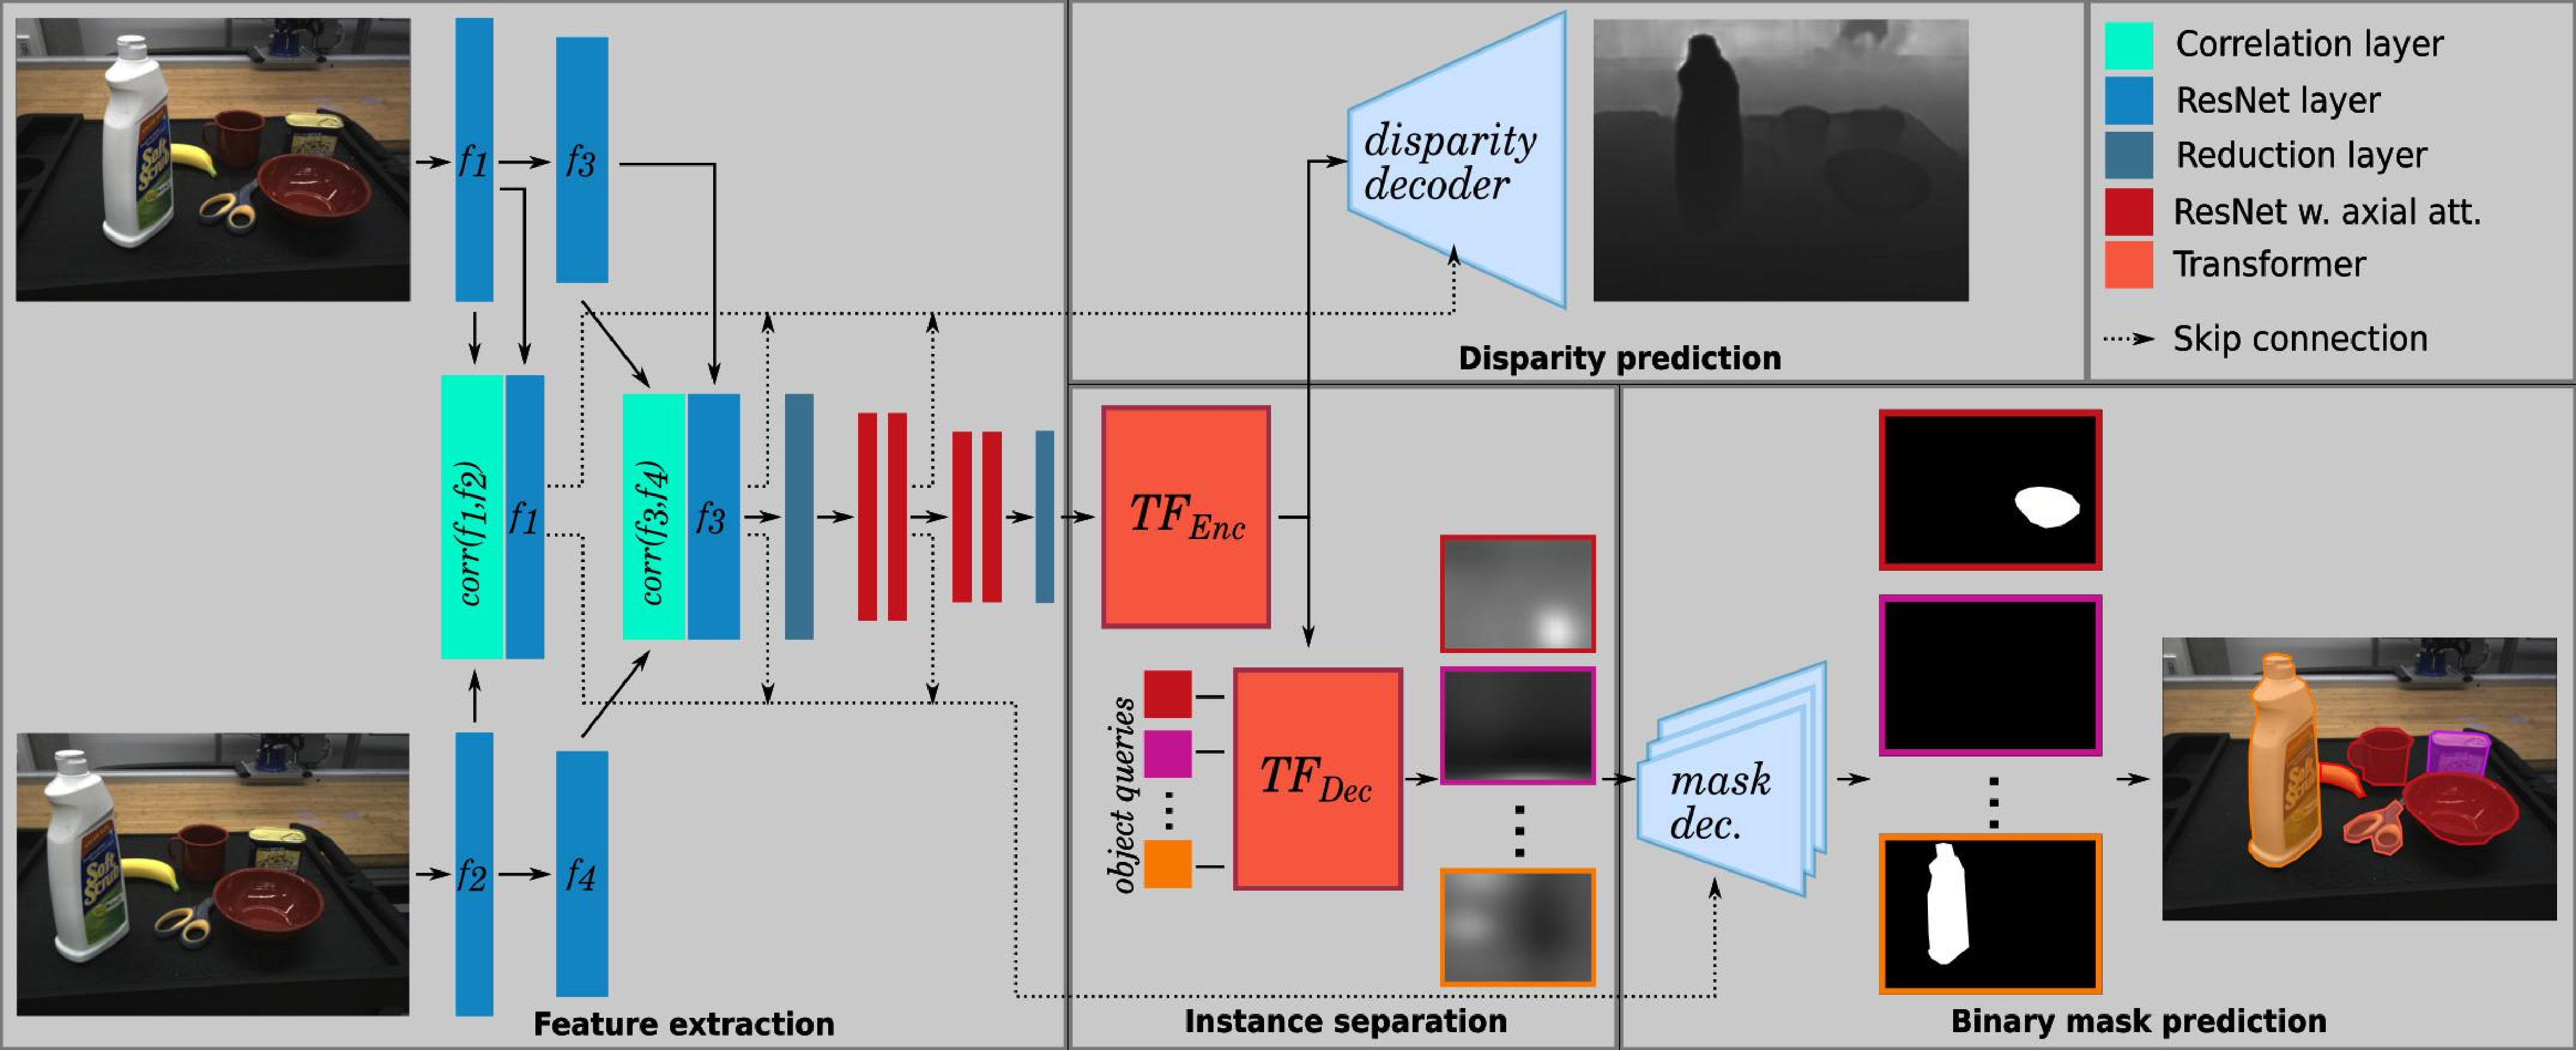
\includegraphics[width=1.\linewidth]{figures/04_setup/arch_final.pdf}
    \caption{INSTR model overview}
    \label{fig:instr}
    
\end{figure}

The INSTR+IoU tracker utilises a matching mechanism with past frame predictions for successful association and track id assignment. More specifically, linear sum assignment with the Hungarian algorithm is performed between the previous and current frame predictions with a threshold for IoU overlap between predicted masks, typically provided as a hyperparameter. This matching mechanism between previous and current frame predicted binary masks results in track id propagation, essentially by reassigning the same track id to the most similar prediction in the current frame. An overview of IoU association matching is provided in Algorithm \ref{alg:iou_matching}.

\begin{algorithm}
\caption{IoU association-based tracking}\label{alg:iou_matching}
\begin{algorithmic}[1]


\While{$t < n_{frames}$}
\State $output_t = forward(inputs_t)$
\If{t >0}
    \State $matched\_output_{t} = hungarian\_matcher(output_t, past\_output)$
    \State $past\_output = matched\_output_{t}$
\Else
    \State $past\_output = output_t$
\EndIf

\EndWhile

\end{algorithmic}
\end{algorithm}

\newpage
It is worth noting that the heuristic based tracker has many limitations and is expected to work well only in scenes with very slow camera movement that result in minimal appearance changes in objects between frames. Since track id propagation is performed based on IoU overlap with predictions from the past frame, any change in appearance that results in an IoU overlap <0.5 between past and current frame prediction results in unsuccessful matching and wrong track id assignment. \par







